\hypertarget{_compute_lstar_8c}{
\section{/home/mgh/LanlGeoMag/libLanlGeoMag/ComputeLstar.c File Reference}
\label{_compute_lstar_8c}\index{/home/mgh/LanlGeoMag/libLanlGeoMag/ComputeLstar.c@{/home/mgh/LanlGeoMag/libLanlGeoMag/ComputeLstar.c}}
}
{\tt \#include $<$stdio.h$>$}\par
{\tt \#include $<$math.h$>$}\par
{\tt \#include \char`\"{}Lgm/Lgm\_\-QuadPack.h\char`\"{}}\par
{\tt \#include \char`\"{}Lgm/Lgm\_\-MagModelInfo.h\char`\"{}}\par
{\tt \#include \char`\"{}Lgm/Lgm\_\-LstarInfo.h\char`\"{}}\par
{\tt \#include $<$gsl/gsl\_\-errno.h$>$}\par
{\tt \#include $<$gsl/gsl\_\-spline.h$>$}\par
{\tt \#include $<$string.h$>$}\par


Include dependency graph for ComputeLstar.c:\nopagebreak
\begin{figure}[H]
\begin{center}
\leavevmode
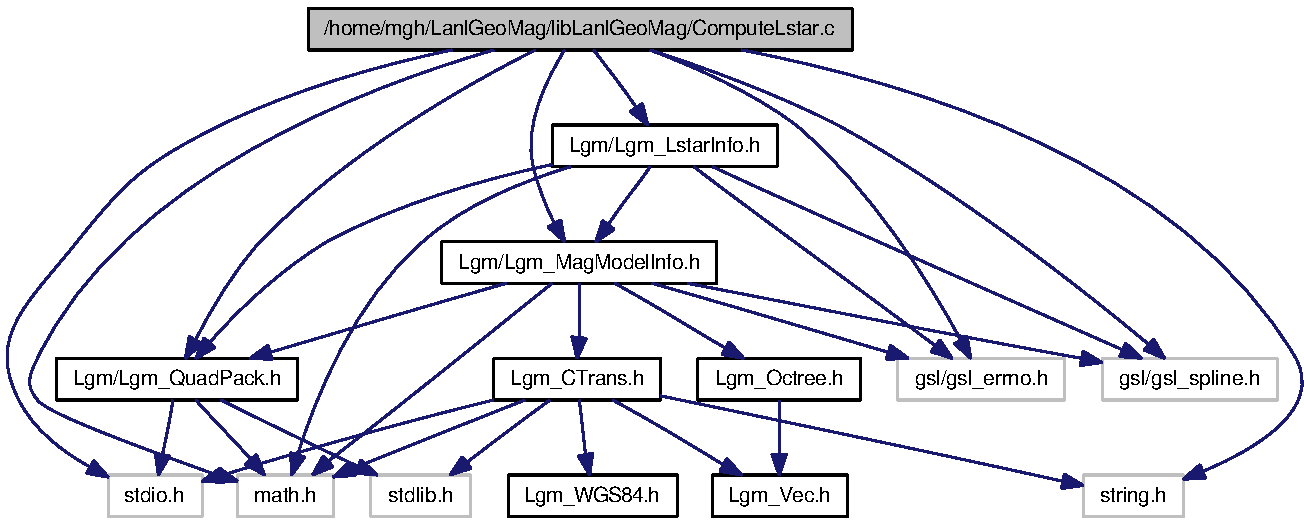
\includegraphics[width=331pt]{_compute_lstar_8c__incl}
\end{center}
\end{figure}
\subsection*{Defines}
\begin{CompactItemize}
\item 
\#define \hyperlink{_compute_lstar_8c_792d250cb395f0b2a568f17662b50b30}{DeltaMLT}~1.0
\end{CompactItemize}
\subsection*{Functions}
\begin{CompactItemize}
\item 
void \hyperlink{_compute_lstar_8c_6b9a47796fc6ddf11d42d91a9885e771}{PredictMlat1} (double $\ast$MirrorMLT, double $\ast$MirrorMlat, int k, double MLT, double $\ast$pred\_\-mlat, double $\ast$pred\_\-delta\_\-mlat, double $\ast$delta)
\item 
void \hyperlink{_compute_lstar_8c_7aae1b668ec7bda0f93ead3c5ecd5429}{PredictMlat2} (double $\ast$MirrorMLT, double $\ast$MirrorMlat, int k, double MLT, double $\ast$pred\_\-mlat, double $\ast$pred\_\-delta\_\-mlat, double $\ast$delta, \hyperlink{struct_lgm___lstar_info}{Lgm\_\-LstarInfo} $\ast$LstarInfo)
\item 
void \hyperlink{_compute_lstar_8c_fbfbd938470e255f3267132c6f96bc48}{SetLstarTolerances} (int Quality, \hyperlink{struct_lgm___lstar_info}{Lgm\_\-LstarInfo} $\ast$s)
\item 
\hyperlink{struct_lgm___lstar_info}{Lgm\_\-LstarInfo} $\ast$ \hyperlink{_compute_lstar_8c_d7d999fbe5d3b065fe808bb3e7ceab0b}{InitLstarInfo} (int VerbosityLevel)
\item 
void \hyperlink{_compute_lstar_8c_a7343c731e76ee9f5190b30a318656f6}{FreeLstarInfo} (\hyperlink{struct_lgm___lstar_info}{Lgm\_\-LstarInfo} $\ast$s)
\item 
\hyperlink{struct_lgm___lstar_info}{Lgm\_\-LstarInfo} $\ast$ \hyperlink{_compute_lstar_8c_84a1ec912704573c21c1e506b72d6f01}{Lgm\_\-CopyLstarInfo} (\hyperlink{struct_lgm___lstar_info}{Lgm\_\-LstarInfo} $\ast$s)
\item 
void \hyperlink{_compute_lstar_8c_68ec464c1b33f0b437d856629f0dd901}{NewTimeLstarInfo} (long int Date, double UT, double PitchAngle, int($\ast$Mag)(\hyperlink{struct_lgm___vector}{Lgm\_\-Vector} $\ast$, \hyperlink{struct_lgm___vector}{Lgm\_\-Vector} $\ast$, \hyperlink{struct_lgm___mag_model_info}{Lgm\_\-MagModelInfo} $\ast$), \hyperlink{struct_lgm___lstar_info}{Lgm\_\-LstarInfo} $\ast$LstarInfo)
\item 
int \hyperlink{_compute_lstar_8c_957a4d60eb4025656b3c2557b402523e}{Lstar} (\hyperlink{struct_lgm___vector}{Lgm\_\-Vector} $\ast$vin, \hyperlink{struct_lgm___lstar_info}{Lgm\_\-LstarInfo} $\ast$LstarInfo)
\item 
double \hyperlink{_compute_lstar_8c_5f75b0909329fb6260c63bc551c29acb}{MagFluxIntegrand} (double Phi, \hyperlink{_lgm___quad_pack_8h_01be5a7db8d2fc2ba26ce793d73b6472}{\_\-qpInfo} $\ast$qpInfo)
\item 
double \hyperlink{_compute_lstar_8c_871565dbd20b1df061fb2e706bd724db}{MagFlux} (\hyperlink{struct_lgm___lstar_info}{Lgm\_\-LstarInfo} $\ast$LstarInfo)
\item 
double \hyperlink{_compute_lstar_8c_fb4cfc3e9728d5ec4867d39f1384dc38}{LambdaIntegrand} (double Lambda, \hyperlink{_lgm___quad_pack_8h_01be5a7db8d2fc2ba26ce793d73b6472}{\_\-qpInfo} $\ast$qpInfo)
\item 
double \hyperlink{_compute_lstar_8c_593bd0ac5cd8b137cbc401b58219df31}{LambdaIntegral} (\hyperlink{struct_lgm___lstar_info}{Lgm\_\-LstarInfo} $\ast$LstarInfo)
\item 
double \hyperlink{_compute_lstar_8c_0f767b7206b1928b2f36fa7c5a26ca33}{MagFluxIntegrand2} (double Phi, \hyperlink{_lgm___quad_pack_8h_01be5a7db8d2fc2ba26ce793d73b6472}{\_\-qpInfo} $\ast$qpInfo)
\item 
double \hyperlink{_compute_lstar_8c_7da6f58b128b4aef809400ada95767d4}{MagFlux2} (\hyperlink{struct_lgm___lstar_info}{Lgm\_\-LstarInfo} $\ast$LstarInfo)
\end{CompactItemize}


\subsection{Define Documentation}
\hypertarget{_compute_lstar_8c_792d250cb395f0b2a568f17662b50b30}{
\index{ComputeLstar.c@{ComputeLstar.c}!DeltaMLT@{DeltaMLT}}
\index{DeltaMLT@{DeltaMLT}!ComputeLstar.c@{ComputeLstar.c}}
\subsubsection[{DeltaMLT}]{\setlength{\rightskip}{0pt plus 5cm}\#define DeltaMLT~1.0}}
\label{_compute_lstar_8c_792d250cb395f0b2a568f17662b50b30}




Definition at line 10 of file ComputeLstar.c.

\subsection{Function Documentation}
\hypertarget{_compute_lstar_8c_6b9a47796fc6ddf11d42d91a9885e771}{
\index{ComputeLstar.c@{ComputeLstar.c}!PredictMlat1@{PredictMlat1}}
\index{PredictMlat1@{PredictMlat1}!ComputeLstar.c@{ComputeLstar.c}}
\subsubsection[{PredictMlat1}]{\setlength{\rightskip}{0pt plus 5cm}void PredictMlat1 (double $\ast$ {\em MirrorMLT}, \/  double $\ast$ {\em MirrorMlat}, \/  int {\em k}, \/  double {\em MLT}, \/  double $\ast$ {\em pred\_\-mlat}, \/  double $\ast$ {\em pred\_\-delta\_\-mlat}, \/  double $\ast$ {\em delta})}}
\label{_compute_lstar_8c_6b9a47796fc6ddf11d42d91a9885e771}




Definition at line 1072 of file ComputeLstar.c.

Here is the call graph for this function:\nopagebreak
\begin{figure}[H]
\begin{center}
\leavevmode
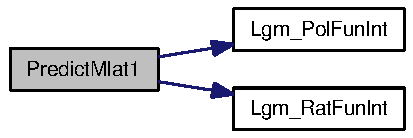
\includegraphics[width=117pt]{_compute_lstar_8c_6b9a47796fc6ddf11d42d91a9885e771_cgraph}
\end{center}
\end{figure}


Here is the caller graph for this function:\nopagebreak
\begin{figure}[H]
\begin{center}
\leavevmode
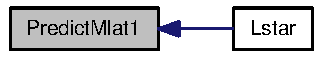
\includegraphics[width=95pt]{_compute_lstar_8c_6b9a47796fc6ddf11d42d91a9885e771_icgraph}
\end{center}
\end{figure}
\hypertarget{_compute_lstar_8c_7aae1b668ec7bda0f93ead3c5ecd5429}{
\index{ComputeLstar.c@{ComputeLstar.c}!PredictMlat2@{PredictMlat2}}
\index{PredictMlat2@{PredictMlat2}!ComputeLstar.c@{ComputeLstar.c}}
\subsubsection[{PredictMlat2}]{\setlength{\rightskip}{0pt plus 5cm}void PredictMlat2 (double $\ast$ {\em MirrorMLT}, \/  double $\ast$ {\em MirrorMlat}, \/  int {\em k}, \/  double {\em MLT}, \/  double $\ast$ {\em pred\_\-mlat}, \/  double $\ast$ {\em pred\_\-delta\_\-mlat}, \/  double $\ast$ {\em delta}, \/  {\bf Lgm\_\-LstarInfo} $\ast$ {\em LstarInfo})}}
\label{_compute_lstar_8c_7aae1b668ec7bda0f93ead3c5ecd5429}




Definition at line 1151 of file ComputeLstar.c.

Here is the call graph for this function:\nopagebreak
\begin{figure}[H]
\begin{center}
\leavevmode
\includegraphics[width=107pt]{_compute_lstar_8c_7aae1b668ec7bda0f93ead3c5ecd5429_cgraph}
\end{center}
\end{figure}


Here is the caller graph for this function:\nopagebreak
\begin{figure}[H]
\begin{center}
\leavevmode
\includegraphics[width=95pt]{_compute_lstar_8c_7aae1b668ec7bda0f93ead3c5ecd5429_icgraph}
\end{center}
\end{figure}
\hypertarget{_compute_lstar_8c_fbfbd938470e255f3267132c6f96bc48}{
\index{ComputeLstar.c@{ComputeLstar.c}!SetLstarTolerances@{SetLstarTolerances}}
\index{SetLstarTolerances@{SetLstarTolerances}!ComputeLstar.c@{ComputeLstar.c}}
\subsubsection[{SetLstarTolerances}]{\setlength{\rightskip}{0pt plus 5cm}void SetLstarTolerances (int {\em Quality}, \/  {\bf Lgm\_\-LstarInfo} $\ast$ {\em s})}}
\label{_compute_lstar_8c_fbfbd938470e255f3267132c6f96bc48}




Definition at line 21 of file ComputeLstar.c.\hypertarget{_compute_lstar_8c_d7d999fbe5d3b065fe808bb3e7ceab0b}{
\index{ComputeLstar.c@{ComputeLstar.c}!InitLstarInfo@{InitLstarInfo}}
\index{InitLstarInfo@{InitLstarInfo}!ComputeLstar.c@{ComputeLstar.c}}
\subsubsection[{InitLstarInfo}]{\setlength{\rightskip}{0pt plus 5cm}{\bf Lgm\_\-LstarInfo}$\ast$ InitLstarInfo (int {\em VerbosityLevel})}}
\label{_compute_lstar_8c_d7d999fbe5d3b065fe808bb3e7ceab0b}




Definition at line 189 of file ComputeLstar.c.

Here is the call graph for this function:\nopagebreak
\begin{figure}[H]
\begin{center}
\leavevmode
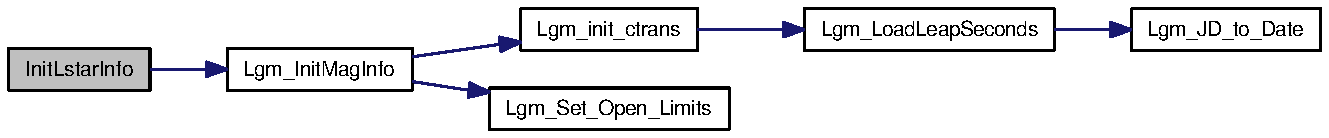
\includegraphics[width=337pt]{_compute_lstar_8c_d7d999fbe5d3b065fe808bb3e7ceab0b_cgraph}
\end{center}
\end{figure}


Here is the caller graph for this function:\nopagebreak
\begin{figure}[H]
\begin{center}
\leavevmode
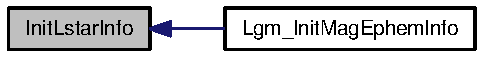
\includegraphics[width=134pt]{_compute_lstar_8c_d7d999fbe5d3b065fe808bb3e7ceab0b_icgraph}
\end{center}
\end{figure}
\hypertarget{_compute_lstar_8c_a7343c731e76ee9f5190b30a318656f6}{
\index{ComputeLstar.c@{ComputeLstar.c}!FreeLstarInfo@{FreeLstarInfo}}
\index{FreeLstarInfo@{FreeLstarInfo}!ComputeLstar.c@{ComputeLstar.c}}
\subsubsection[{FreeLstarInfo}]{\setlength{\rightskip}{0pt plus 5cm}void FreeLstarInfo ({\bf Lgm\_\-LstarInfo} $\ast$ {\em s})}}
\label{_compute_lstar_8c_a7343c731e76ee9f5190b30a318656f6}




Definition at line 221 of file ComputeLstar.c.

Here is the call graph for this function:\nopagebreak
\begin{figure}[H]
\begin{center}
\leavevmode
\includegraphics[width=188pt]{_compute_lstar_8c_a7343c731e76ee9f5190b30a318656f6_cgraph}
\end{center}
\end{figure}


Here is the caller graph for this function:\nopagebreak
\begin{figure}[H]
\begin{center}
\leavevmode
\includegraphics[width=140pt]{_compute_lstar_8c_a7343c731e76ee9f5190b30a318656f6_icgraph}
\end{center}
\end{figure}
\hypertarget{_compute_lstar_8c_84a1ec912704573c21c1e506b72d6f01}{
\index{ComputeLstar.c@{ComputeLstar.c}!Lgm\_\-CopyLstarInfo@{Lgm\_\-CopyLstarInfo}}
\index{Lgm\_\-CopyLstarInfo@{Lgm\_\-CopyLstarInfo}!ComputeLstar.c@{ComputeLstar.c}}
\subsubsection[{Lgm\_\-CopyLstarInfo}]{\setlength{\rightskip}{0pt plus 5cm}{\bf Lgm\_\-LstarInfo}$\ast$ Lgm\_\-CopyLstarInfo ({\bf Lgm\_\-LstarInfo} $\ast$ {\em s})}}
\label{_compute_lstar_8c_84a1ec912704573c21c1e506b72d6f01}




Definition at line 235 of file ComputeLstar.c.

Here is the call graph for this function:\nopagebreak
\begin{figure}[H]
\begin{center}
\leavevmode
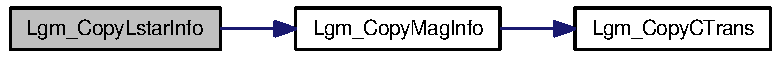
\includegraphics[width=205pt]{_compute_lstar_8c_84a1ec912704573c21c1e506b72d6f01_cgraph}
\end{center}
\end{figure}
\hypertarget{_compute_lstar_8c_68ec464c1b33f0b437d856629f0dd901}{
\index{ComputeLstar.c@{ComputeLstar.c}!NewTimeLstarInfo@{NewTimeLstarInfo}}
\index{NewTimeLstarInfo@{NewTimeLstarInfo}!ComputeLstar.c@{ComputeLstar.c}}
\subsubsection[{NewTimeLstarInfo}]{\setlength{\rightskip}{0pt plus 5cm}void NewTimeLstarInfo (long int {\em Date}, \/  double {\em UT}, \/  double {\em PitchAngle}, \/  int($\ast$)({\bf Lgm\_\-Vector} $\ast$, {\bf Lgm\_\-Vector} $\ast$, {\bf Lgm\_\-MagModelInfo} $\ast$) {\em Mag}, \/  {\bf Lgm\_\-LstarInfo} $\ast$ {\em LstarInfo})}}
\label{_compute_lstar_8c_68ec464c1b33f0b437d856629f0dd901}




Definition at line 281 of file ComputeLstar.c.

Here is the call graph for this function:\nopagebreak
\begin{figure}[H]
\begin{center}
\leavevmode
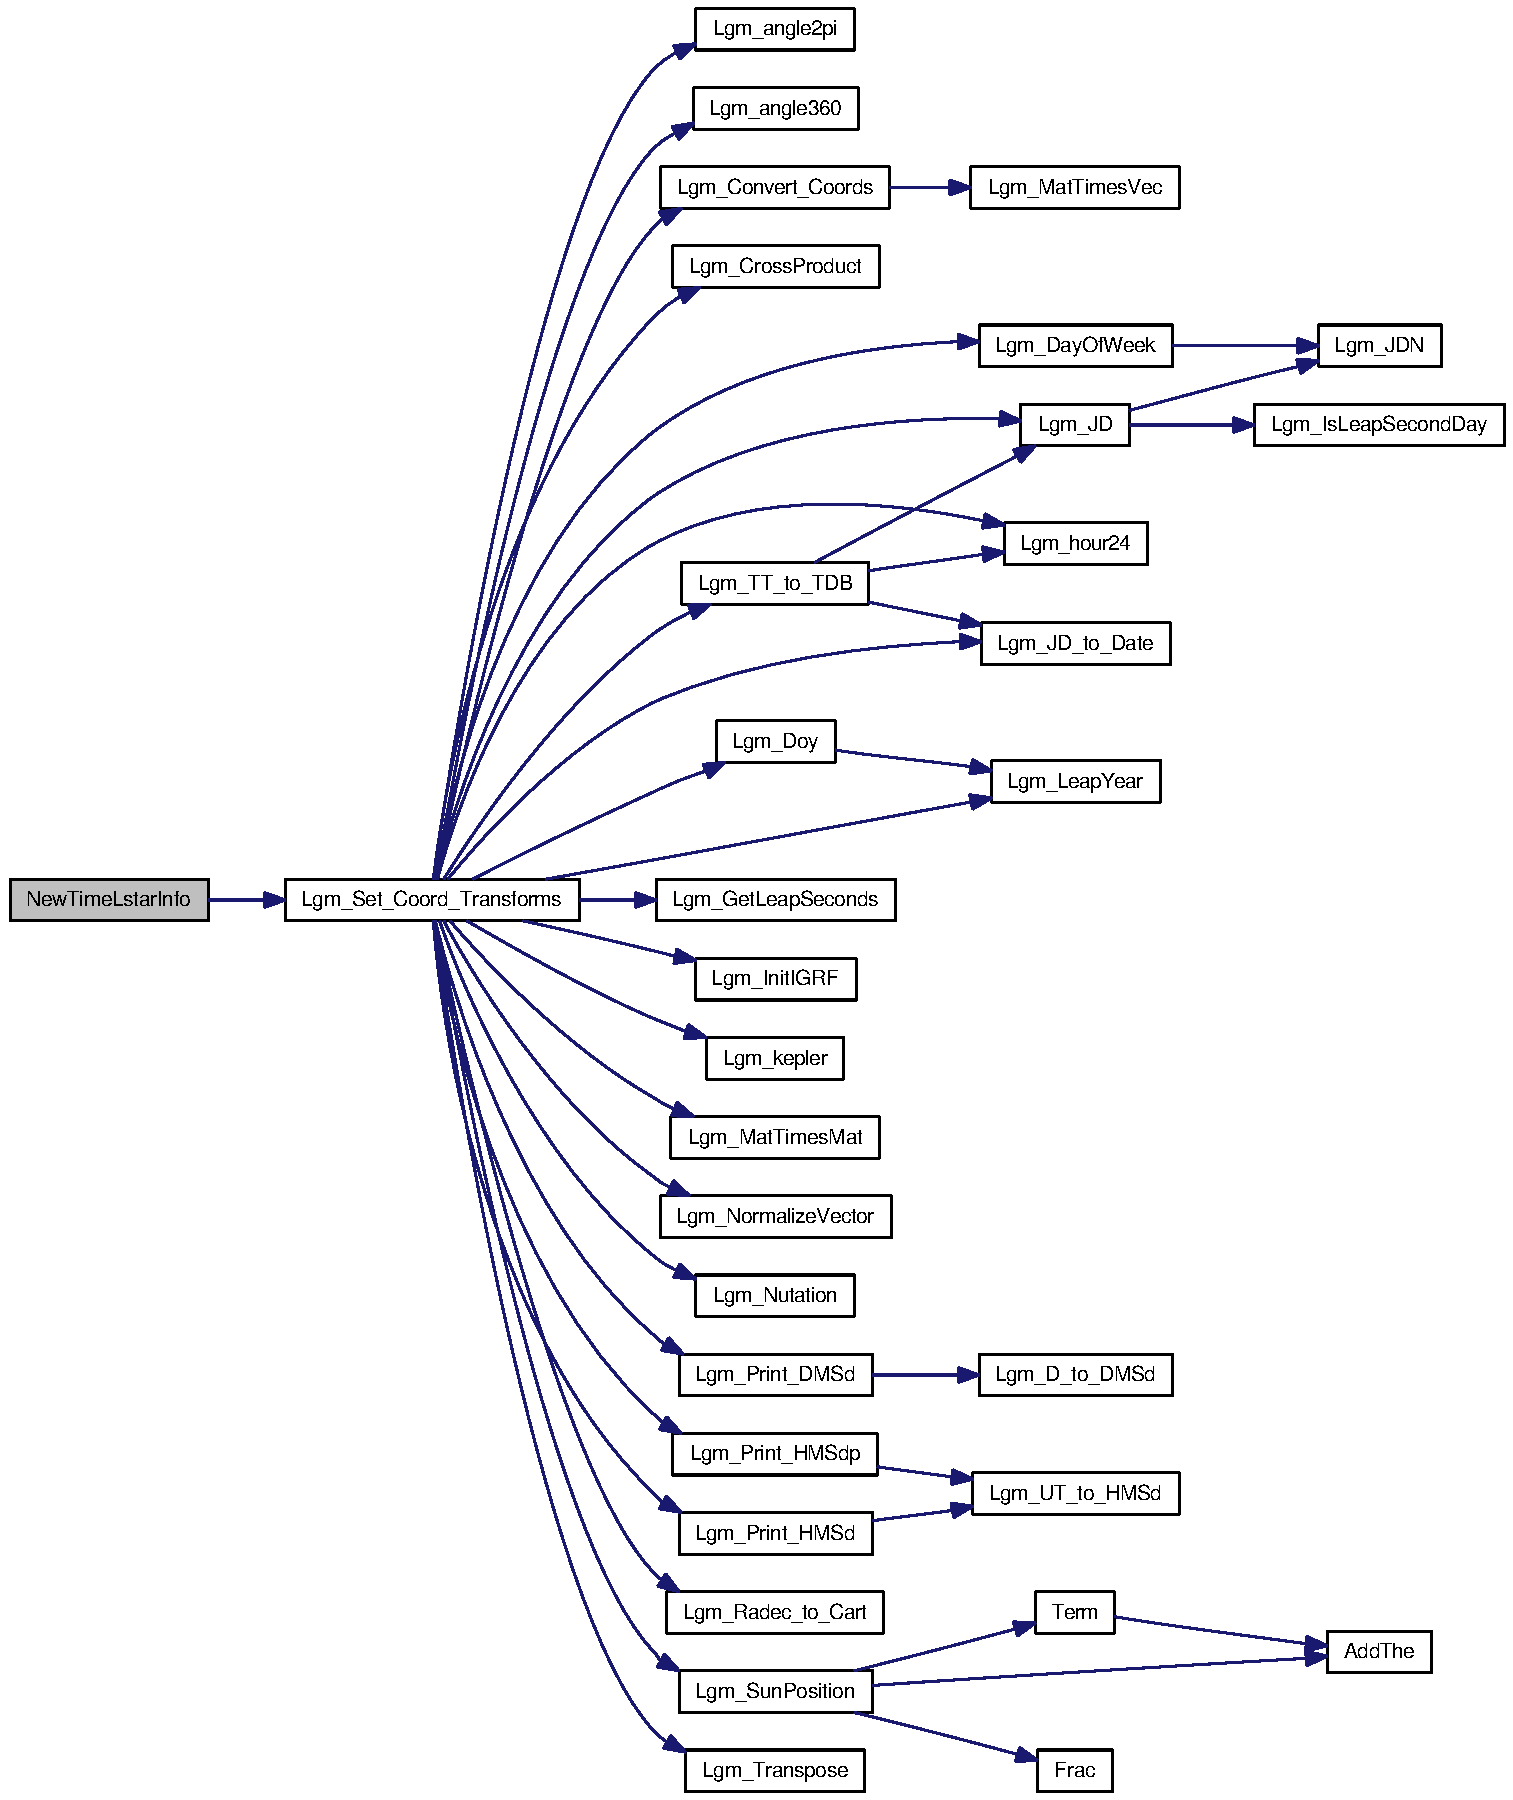
\includegraphics[width=381pt]{_compute_lstar_8c_68ec464c1b33f0b437d856629f0dd901_cgraph}
\end{center}
\end{figure}
\hypertarget{_compute_lstar_8c_957a4d60eb4025656b3c2557b402523e}{
\index{ComputeLstar.c@{ComputeLstar.c}!Lstar@{Lstar}}
\index{Lstar@{Lstar}!ComputeLstar.c@{ComputeLstar.c}}
\subsubsection[{Lstar}]{\setlength{\rightskip}{0pt plus 5cm}int Lstar ({\bf Lgm\_\-Vector} $\ast$ {\em vin}, \/  {\bf Lgm\_\-LstarInfo} $\ast$ {\em LstarInfo})}}
\label{_compute_lstar_8c_957a4d60eb4025656b3c2557b402523e}




Definition at line 307 of file ComputeLstar.c.

Here is the call graph for this function:\nopagebreak
\begin{figure}[H]
\begin{center}
\leavevmode
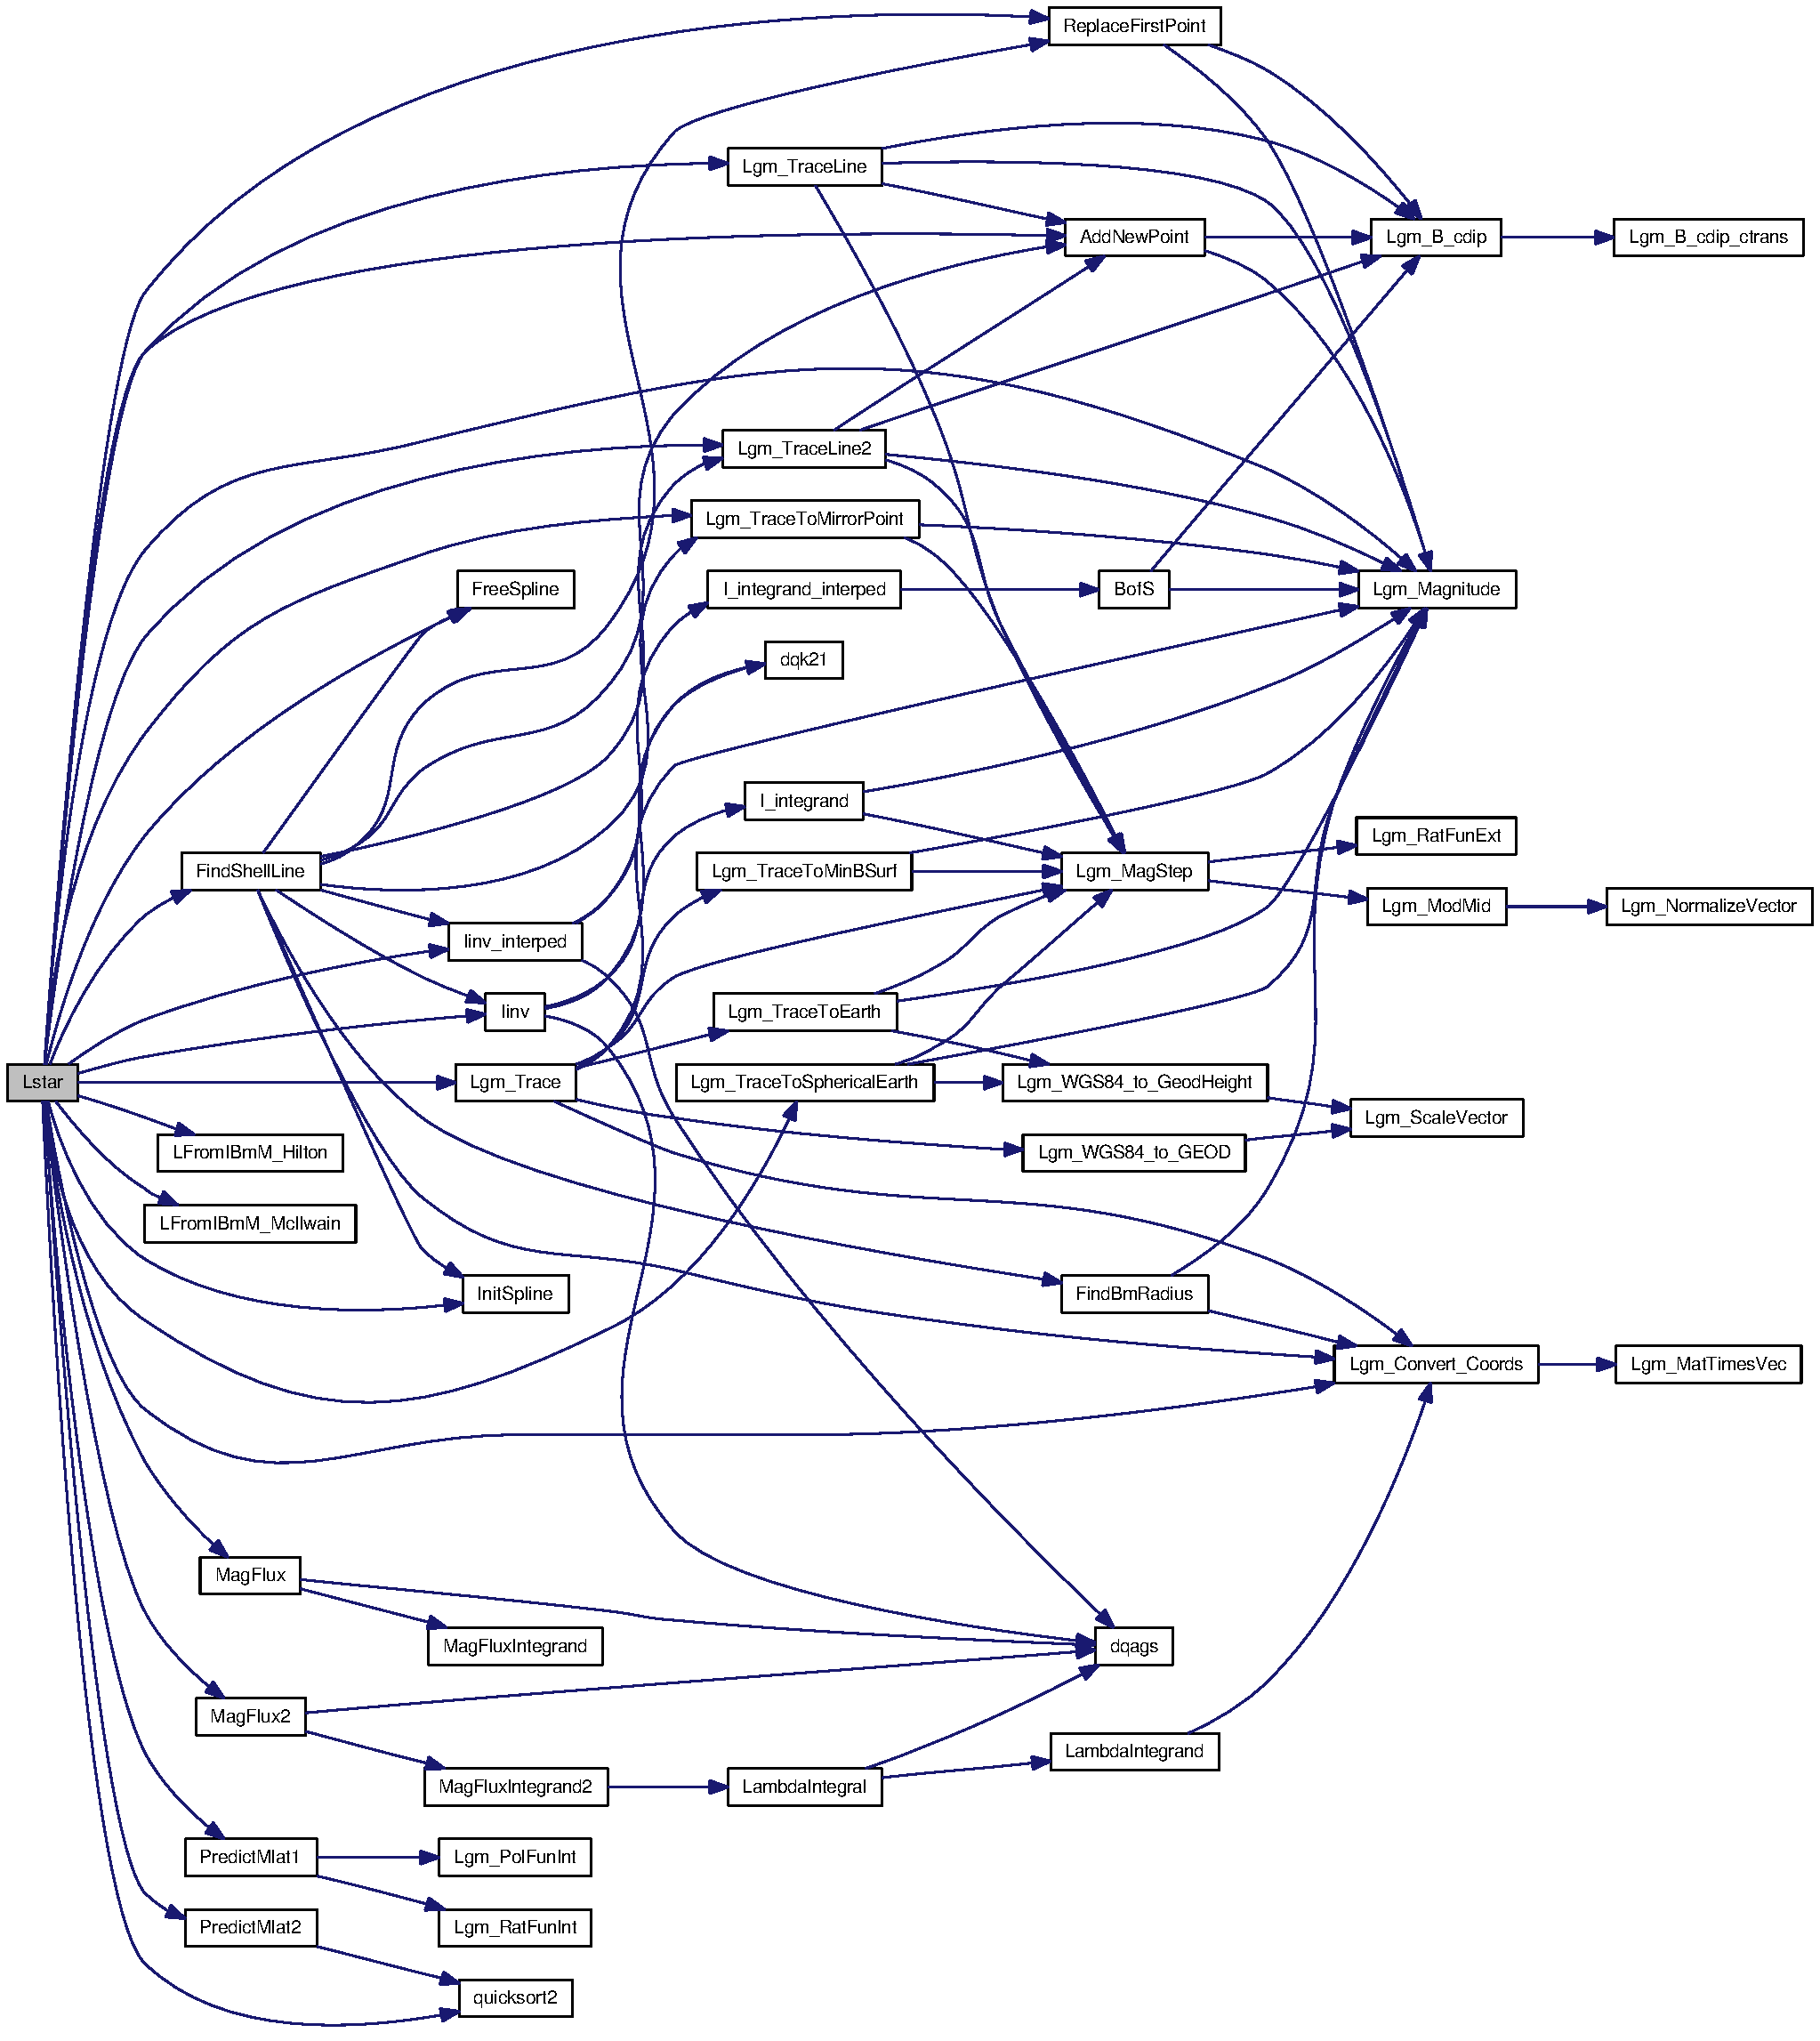
\includegraphics[width=420pt]{_compute_lstar_8c_957a4d60eb4025656b3c2557b402523e_cgraph}
\end{center}
\end{figure}
\hypertarget{_compute_lstar_8c_5f75b0909329fb6260c63bc551c29acb}{
\index{ComputeLstar.c@{ComputeLstar.c}!MagFluxIntegrand@{MagFluxIntegrand}}
\index{MagFluxIntegrand@{MagFluxIntegrand}!ComputeLstar.c@{ComputeLstar.c}}
\subsubsection[{MagFluxIntegrand}]{\setlength{\rightskip}{0pt plus 5cm}double MagFluxIntegrand (double {\em Phi}, \/  {\bf \_\-qpInfo} $\ast$ {\em qpInfo})}}
\label{_compute_lstar_8c_5f75b0909329fb6260c63bc551c29acb}




Definition at line 815 of file ComputeLstar.c.

Here is the caller graph for this function:\nopagebreak
\begin{figure}[H]
\begin{center}
\leavevmode
\includegraphics[width=151pt]{_compute_lstar_8c_5f75b0909329fb6260c63bc551c29acb_icgraph}
\end{center}
\end{figure}
\hypertarget{_compute_lstar_8c_871565dbd20b1df061fb2e706bd724db}{
\index{ComputeLstar.c@{ComputeLstar.c}!MagFlux@{MagFlux}}
\index{MagFlux@{MagFlux}!ComputeLstar.c@{ComputeLstar.c}}
\subsubsection[{MagFlux}]{\setlength{\rightskip}{0pt plus 5cm}double MagFlux ({\bf Lgm\_\-LstarInfo} $\ast$ {\em LstarInfo})}}
\label{_compute_lstar_8c_871565dbd20b1df061fb2e706bd724db}




Definition at line 842 of file ComputeLstar.c.

Here is the call graph for this function:\nopagebreak
\begin{figure}[H]
\begin{center}
\leavevmode
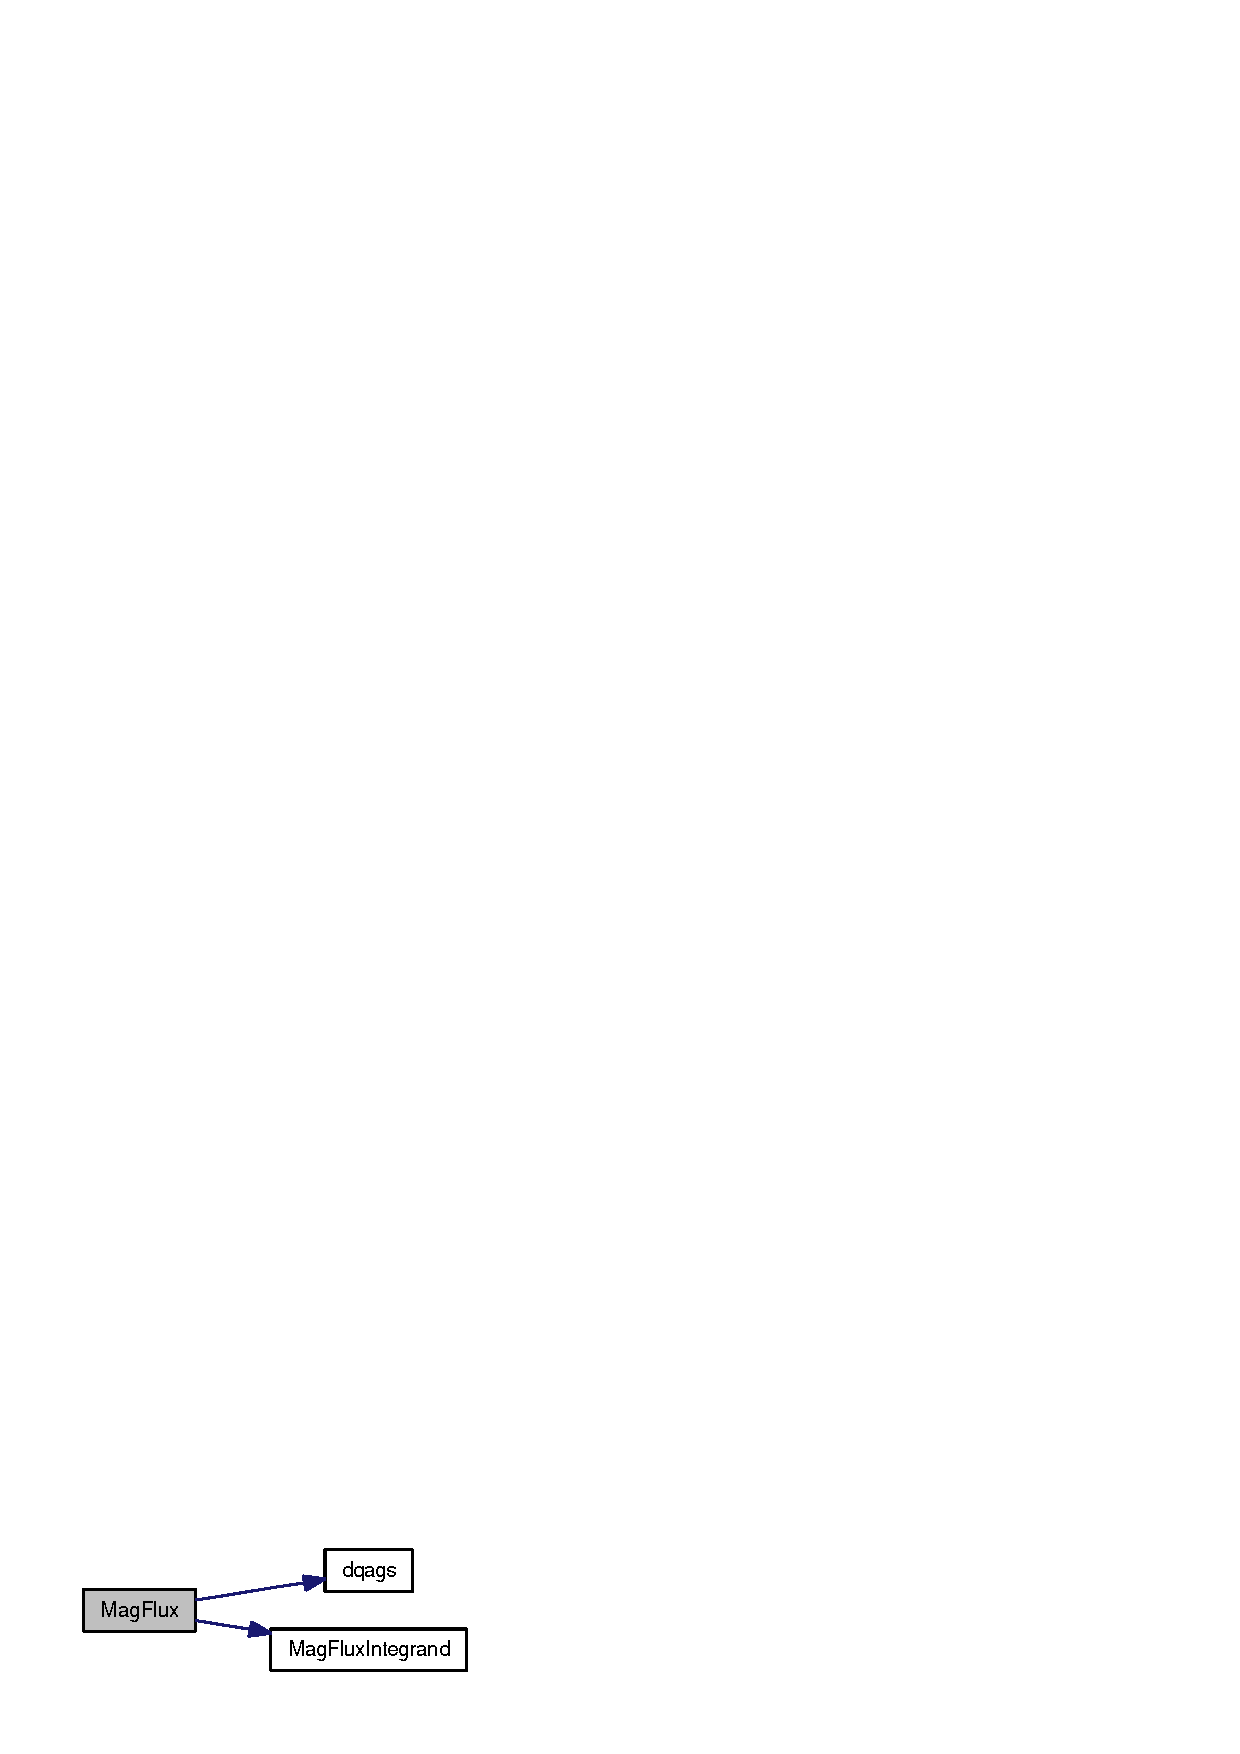
\includegraphics[width=114pt]{_compute_lstar_8c_871565dbd20b1df061fb2e706bd724db_cgraph}
\end{center}
\end{figure}


Here is the caller graph for this function:\nopagebreak
\begin{figure}[H]
\begin{center}
\leavevmode
\includegraphics[width=86pt]{_compute_lstar_8c_871565dbd20b1df061fb2e706bd724db_icgraph}
\end{center}
\end{figure}
\hypertarget{_compute_lstar_8c_fb4cfc3e9728d5ec4867d39f1384dc38}{
\index{ComputeLstar.c@{ComputeLstar.c}!LambdaIntegrand@{LambdaIntegrand}}
\index{LambdaIntegrand@{LambdaIntegrand}!ComputeLstar.c@{ComputeLstar.c}}
\subsubsection[{LambdaIntegrand}]{\setlength{\rightskip}{0pt plus 5cm}double LambdaIntegrand (double {\em Lambda}, \/  {\bf \_\-qpInfo} $\ast$ {\em qpInfo})}}
\label{_compute_lstar_8c_fb4cfc3e9728d5ec4867d39f1384dc38}




Definition at line 909 of file ComputeLstar.c.

Here is the call graph for this function:\nopagebreak
\begin{figure}[H]
\begin{center}
\leavevmode
\includegraphics[width=209pt]{_compute_lstar_8c_fb4cfc3e9728d5ec4867d39f1384dc38_cgraph}
\end{center}
\end{figure}


Here is the caller graph for this function:\nopagebreak
\begin{figure}[H]
\begin{center}
\leavevmode
\includegraphics[width=281pt]{_compute_lstar_8c_fb4cfc3e9728d5ec4867d39f1384dc38_icgraph}
\end{center}
\end{figure}
\hypertarget{_compute_lstar_8c_593bd0ac5cd8b137cbc401b58219df31}{
\index{ComputeLstar.c@{ComputeLstar.c}!LambdaIntegral@{LambdaIntegral}}
\index{LambdaIntegral@{LambdaIntegral}!ComputeLstar.c@{ComputeLstar.c}}
\subsubsection[{LambdaIntegral}]{\setlength{\rightskip}{0pt plus 5cm}double LambdaIntegral ({\bf Lgm\_\-LstarInfo} $\ast$ {\em LstarInfo})}}
\label{_compute_lstar_8c_593bd0ac5cd8b137cbc401b58219df31}




Definition at line 945 of file ComputeLstar.c.

Here is the call graph for this function:\nopagebreak
\begin{figure}[H]
\begin{center}
\leavevmode
\includegraphics[width=269pt]{_compute_lstar_8c_593bd0ac5cd8b137cbc401b58219df31_cgraph}
\end{center}
\end{figure}


Here is the caller graph for this function:\nopagebreak
\begin{figure}[H]
\begin{center}
\leavevmode
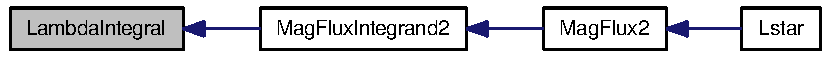
\includegraphics[width=217pt]{_compute_lstar_8c_593bd0ac5cd8b137cbc401b58219df31_icgraph}
\end{center}
\end{figure}
\hypertarget{_compute_lstar_8c_0f767b7206b1928b2f36fa7c5a26ca33}{
\index{ComputeLstar.c@{ComputeLstar.c}!MagFluxIntegrand2@{MagFluxIntegrand2}}
\index{MagFluxIntegrand2@{MagFluxIntegrand2}!ComputeLstar.c@{ComputeLstar.c}}
\subsubsection[{MagFluxIntegrand2}]{\setlength{\rightskip}{0pt plus 5cm}double MagFluxIntegrand2 (double {\em Phi}, \/  {\bf \_\-qpInfo} $\ast$ {\em qpInfo})}}
\label{_compute_lstar_8c_0f767b7206b1928b2f36fa7c5a26ca33}




Definition at line 1005 of file ComputeLstar.c.

Here is the call graph for this function:\nopagebreak
\begin{figure}[H]
\begin{center}
\leavevmode
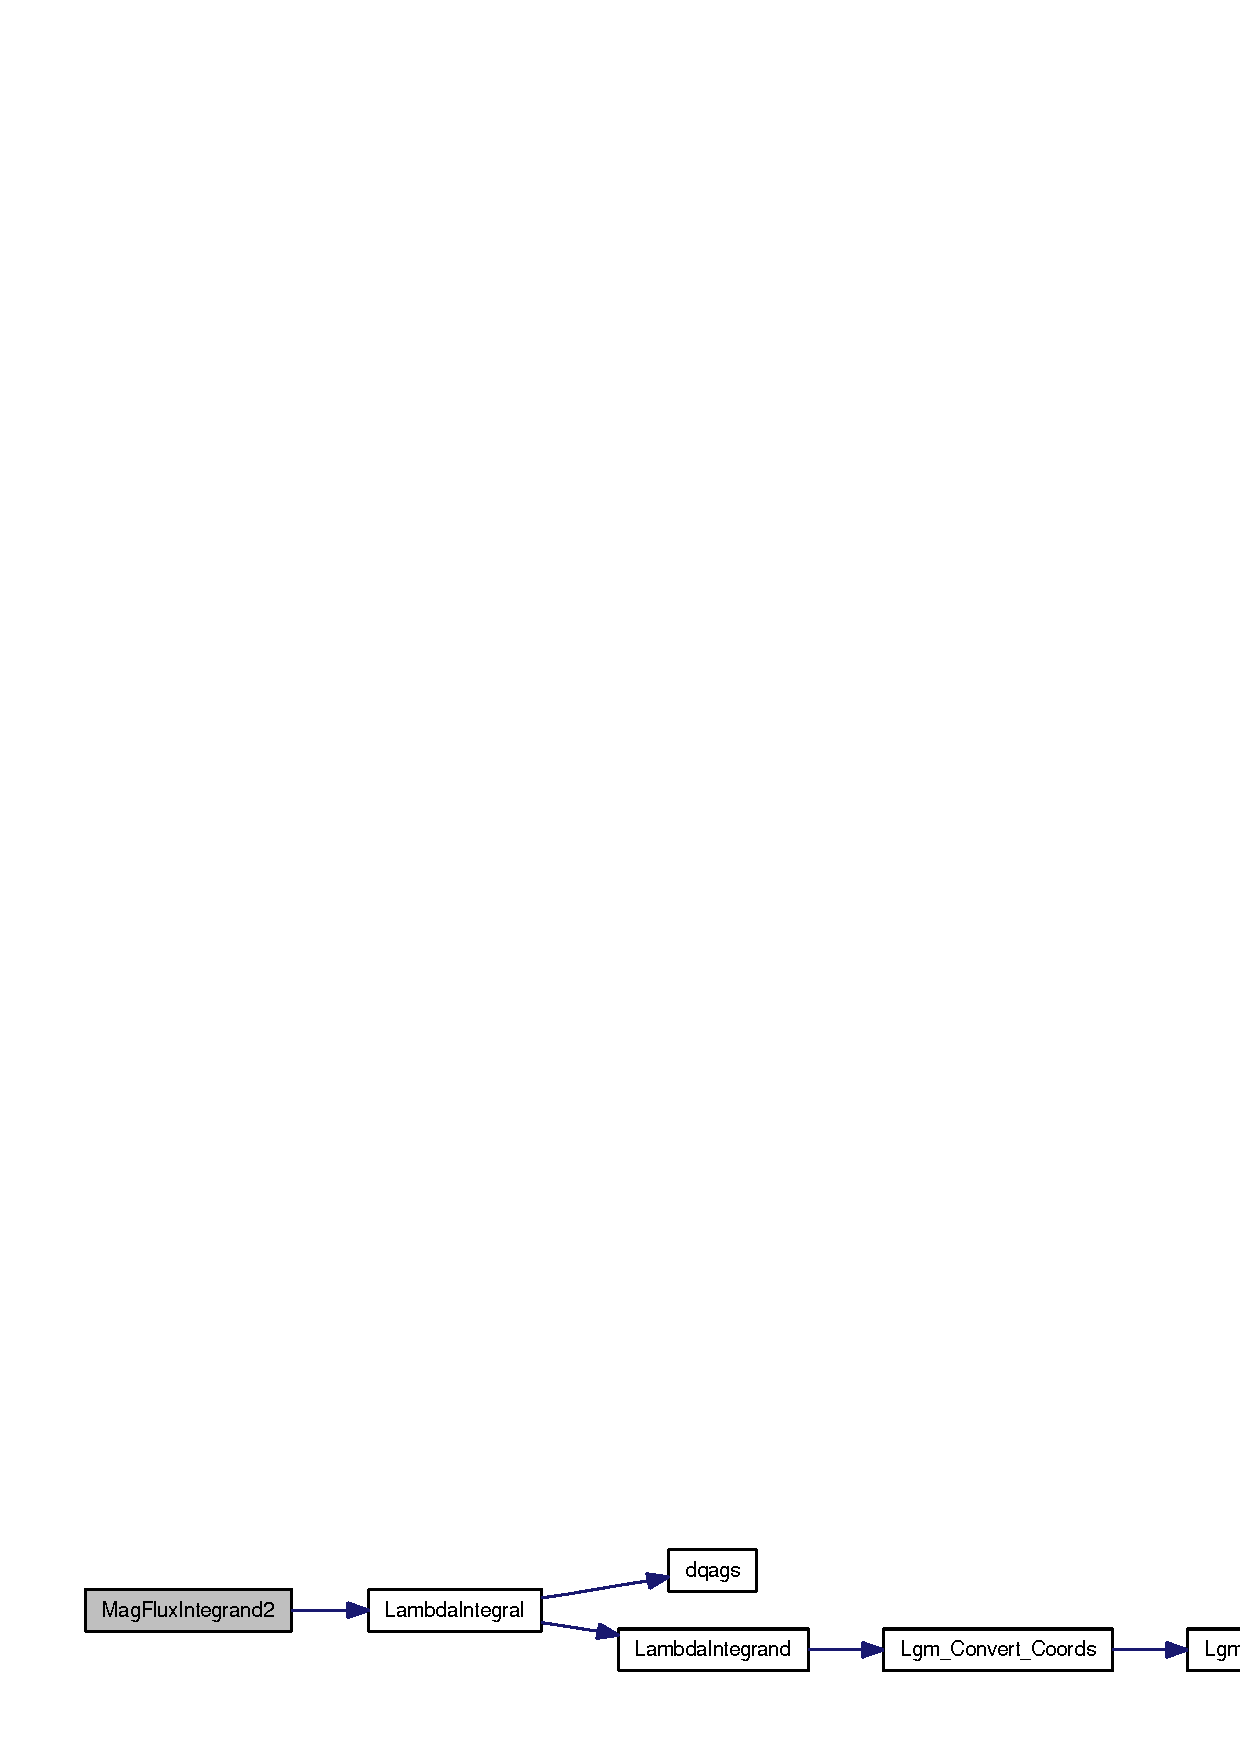
\includegraphics[width=337pt]{_compute_lstar_8c_0f767b7206b1928b2f36fa7c5a26ca33_cgraph}
\end{center}
\end{figure}


Here is the caller graph for this function:\nopagebreak
\begin{figure}[H]
\begin{center}
\leavevmode
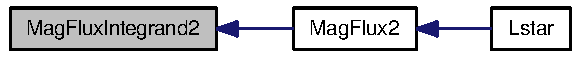
\includegraphics[width=157pt]{_compute_lstar_8c_0f767b7206b1928b2f36fa7c5a26ca33_icgraph}
\end{center}
\end{figure}
\hypertarget{_compute_lstar_8c_7da6f58b128b4aef809400ada95767d4}{
\index{ComputeLstar.c@{ComputeLstar.c}!MagFlux2@{MagFlux2}}
\index{MagFlux2@{MagFlux2}!ComputeLstar.c@{ComputeLstar.c}}
\subsubsection[{MagFlux2}]{\setlength{\rightskip}{0pt plus 5cm}double MagFlux2 ({\bf Lgm\_\-LstarInfo} $\ast$ {\em LstarInfo})}}
\label{_compute_lstar_8c_7da6f58b128b4aef809400ada95767d4}




Definition at line 1023 of file ComputeLstar.c.

Here is the call graph for this function:\nopagebreak
\begin{figure}[H]
\begin{center}
\leavevmode
\includegraphics[width=385pt]{_compute_lstar_8c_7da6f58b128b4aef809400ada95767d4_cgraph}
\end{center}
\end{figure}


Here is the caller graph for this function:\nopagebreak
\begin{figure}[H]
\begin{center}
\leavevmode
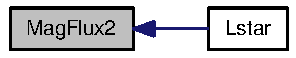
\includegraphics[width=89pt]{_compute_lstar_8c_7da6f58b128b4aef809400ada95767d4_icgraph}
\end{center}
\end{figure}
